\BigLetter{T}{he} benchmarks for the combined BDAE and \CodeName framework will primarily focus on two real world data and computationally heavy applications in big data analysis and image processing namely; Computed Tomographic (CT) reconstruction and Circle detection.
\newline

The benchmarks are executed on an Ubuntu 14.04 LTS (Trusty Tahr)\cite{PageUbuntu1404} cluster with 8 nodes each with following specifications:
\vspace*{5mm}
\begin{table}[h!]
	\centering
	\begin{tabular}{l l}
		\textbf{CPU} & AMD Opteron 6272 \emph{Interlagos} \\
		\textbf{Processor frequency (GHz)} & 2.1 \\
		\textbf{\# cores} & 32 (dual socket) \\
		\textbf{Memory (GB)} & 128 \\
		\textbf{SSD Storage (GB)} & 128 
	\end{tabular}
	\caption{Environment specifications.\label{tab:specifications}}
\end{table}

\section{CT reconstruction}
In the healthcare industry tomographic imaging is widely used for confirming injuries such as broken bones. The reconstruction (Figure \ref{fig:ct}) can be simulated by a mathematical model for transforming a series of at least 180 degrees\footnote{The rest of the 180 degrees is simply a mirror of the others.} of 2D images (\textit{projections}) into a 3D volume (\textit{reconstruction}).
\newpage

\begin{figure}
	\vspace*{3mm}
	\centering
	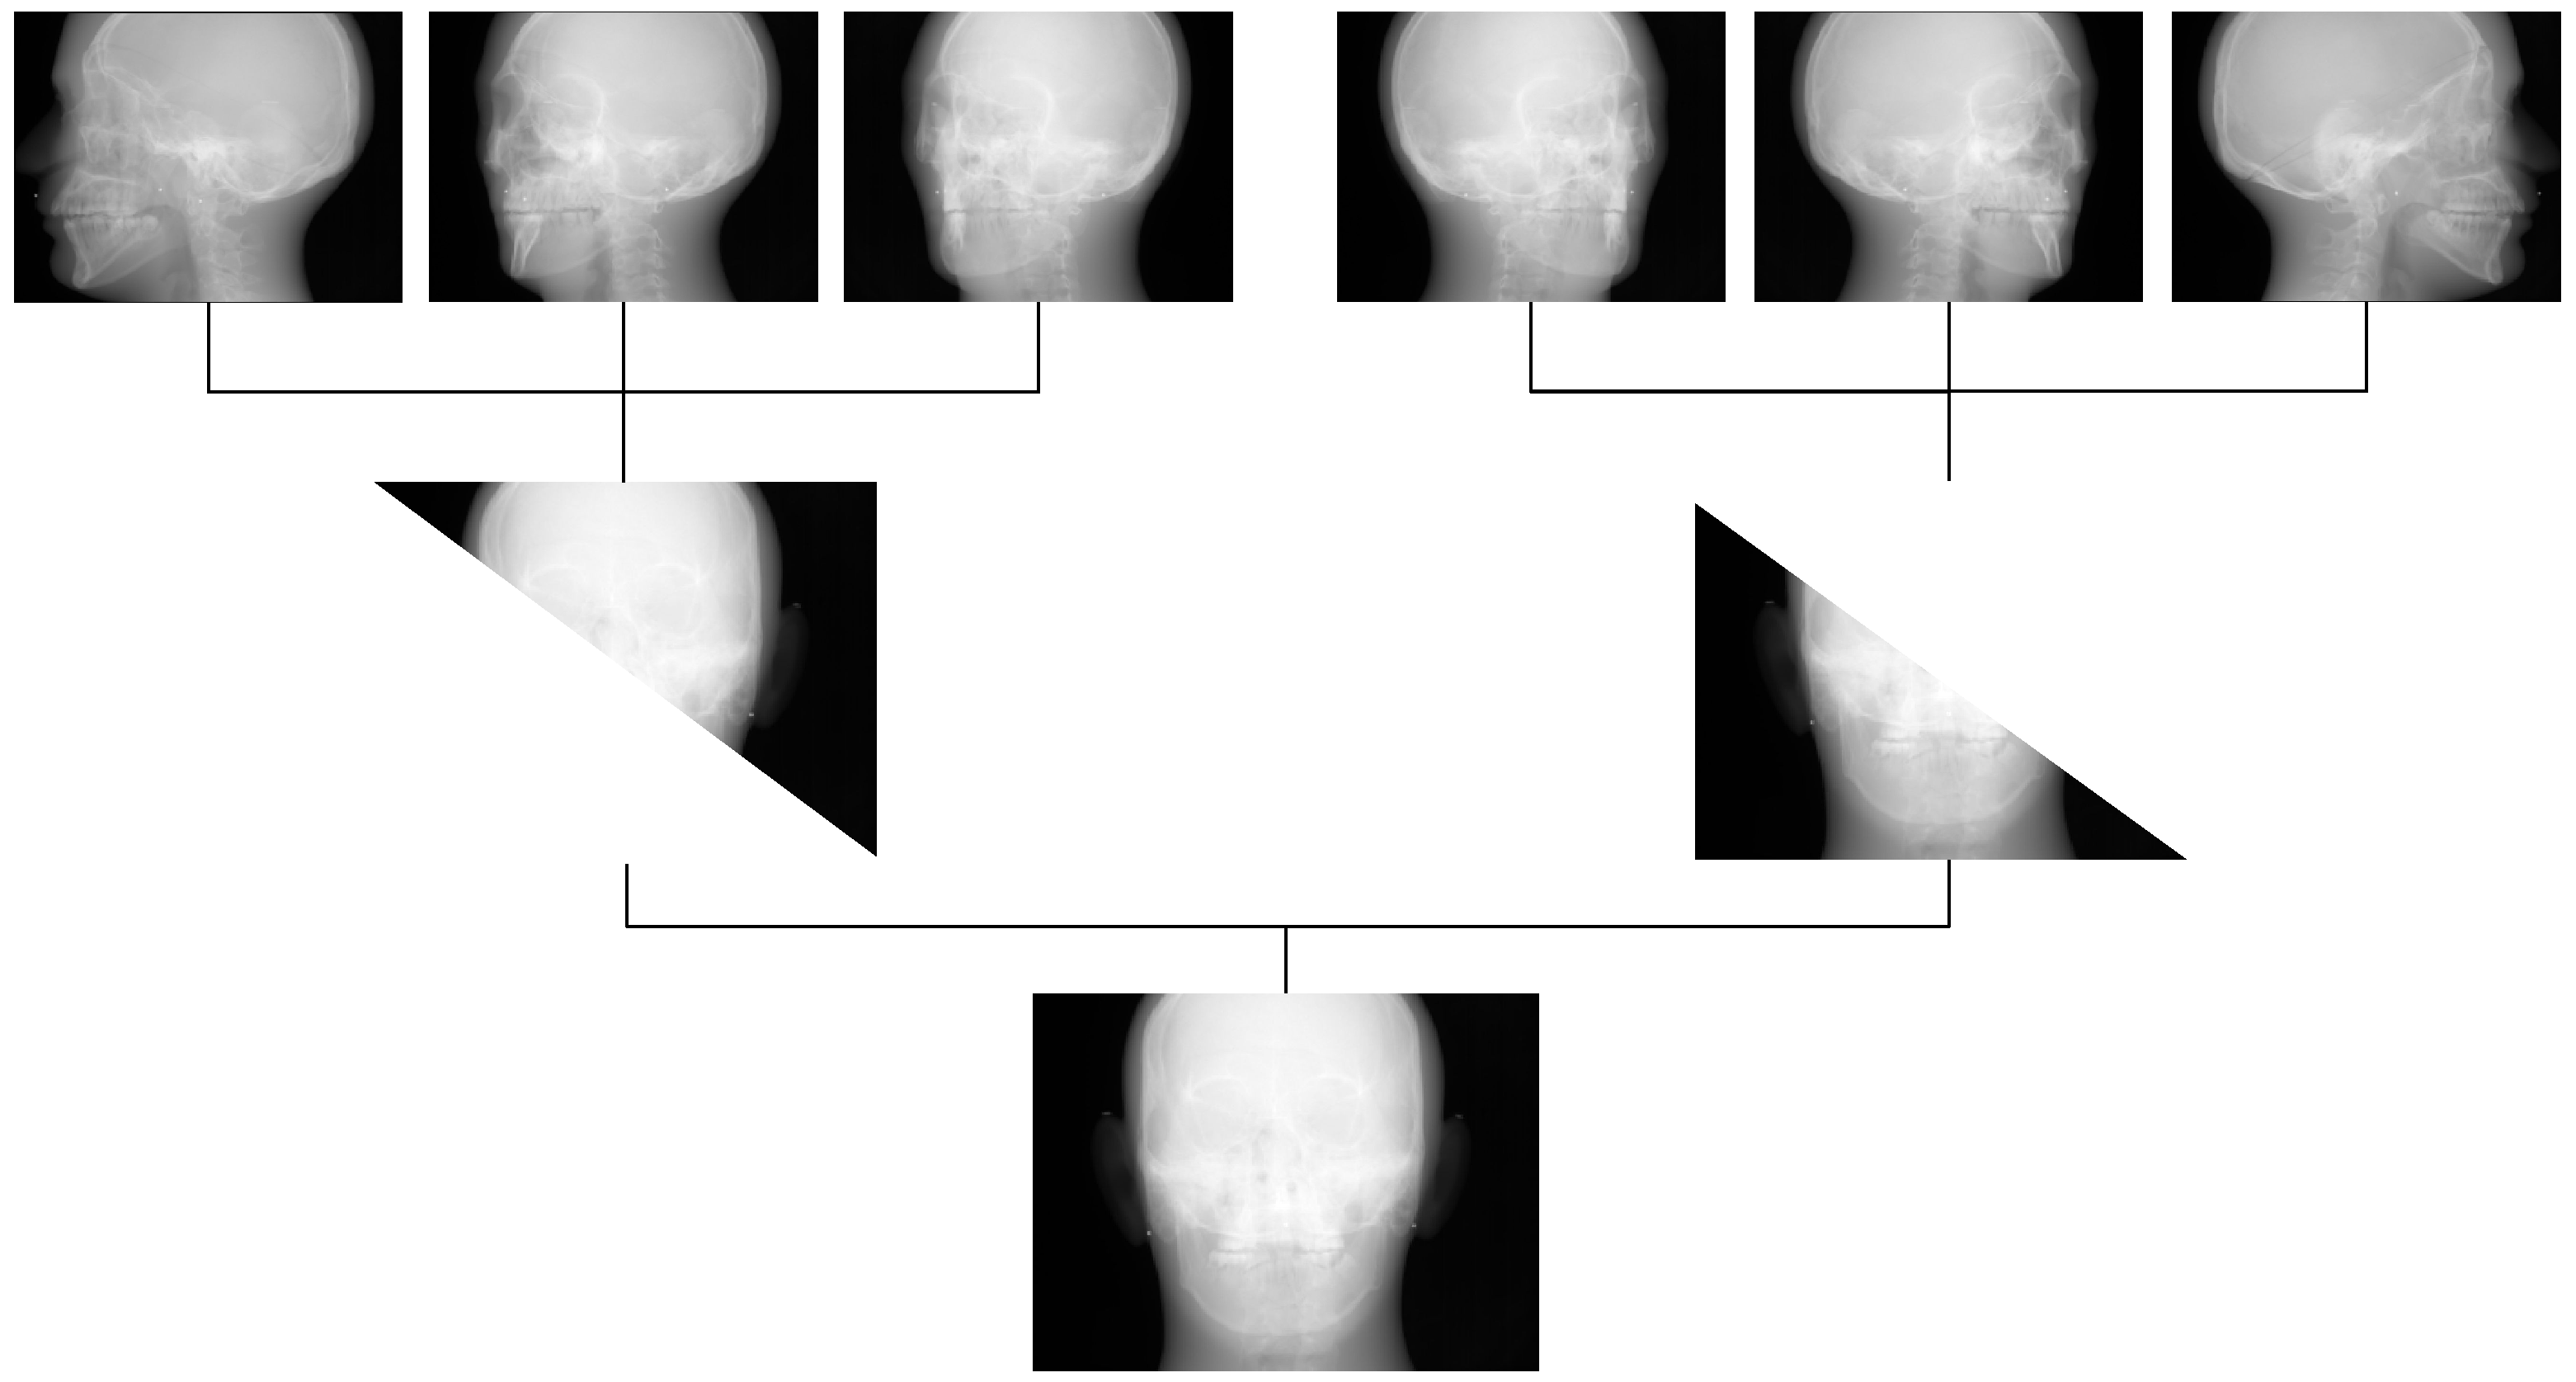
\includegraphics[scale=0.25]{pdf/CT.pdf}
	\caption[]{An example of a distributed parallel CT reconstruction where the second (middle) step is a simulated result to illustrate the notion of a partial volume. \label{fig:ct}}
	\vspace*{3mm}
\end{figure}

\noindent
Simulation results are computed by the cone-beam step-and-shoot method based on the inverse Radon transform known as the filtered back projection algorithm which requires several steps. This benchmark, however, is a simplified version that concentrates on the primary part of the calculation using following precalculated values and partial results:

\begin{itemize}
	\item Preprocessed 2D projects.
	\item Combination of all \texttt{(x, y)} coordinates for the resulting 3D volume.
	\item \texttt{z} coordinates for the 3D volume.
	\item Mapping between 3D and 2D coordinates.
	\item Compensating weights for the cone-beam effect.
\end{itemize}

\subsection*{Simulation results}
The sequential implementation of the CT reconstruction simulation is used as a baseline for calculating the speedup based on the runtime from executing it using the BDAE and \CodeName framework.
\newpage

The sequential source code is rewritten using the Numpy array template (Section \ref{sec:templates}) based on the BDAE \texttt{MapReduceDataset}. The 2D projections are loaded as part of the preprocessing step (Section \ref{sec:sofabaseobject}) and distributed using the chosen distribution strategy.

\begin{itemize}
	\item The \texttt{map} function is basically the sequential code with a reduced number of iterations\footnote{Based on the distribution strategy and the number of storage nodes}.
	\item The \texttt{reduce} function reduces the partial results by applying a universal add operation recursively along the required axis.
\end{itemize}

The CT reconstruction code is executed on three different datasets in increasing volume, and the expectations for the results are that the performance of BDAE will rise the larger the data. Figure \ref{fig:fdk-speedup} presents the speedup results of BDAE compared to the sequential implementation of the CT reconstruction (Graphs of the execution times are in Appendix \ref{app:fdk}).

\begin{figure}[h!]
	\centering
	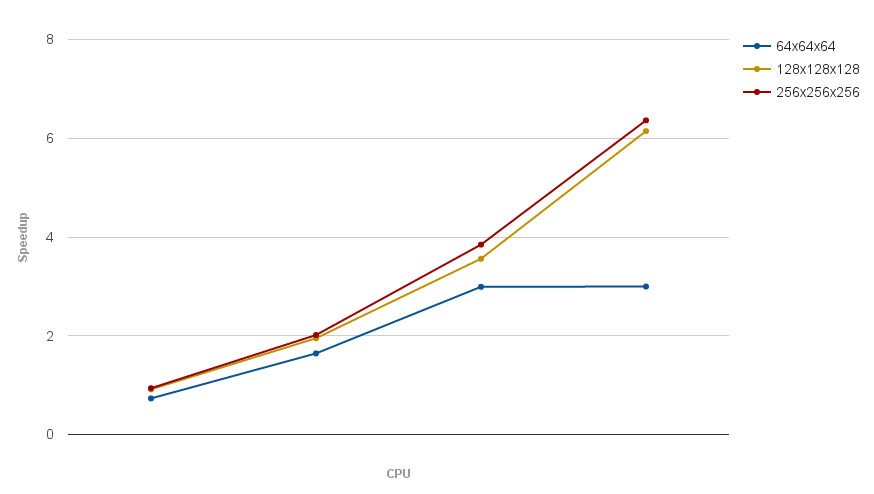
\includegraphics[scale=0.4]{img/fdk-speedup.png}
	\caption[]{Speedup gained using BDAE on the three different datasets. \label{fig:fdk-speedup}}
\end{figure}

The speedup gained is constant using four or more storage nodes on the small 64x64x64 voxels dataset as expected, this is due to the network communication overhead which is dominating the combined execution time. Otherwise, the speedup is quite satisfactory considering the fact that the communication protocol is based on the pure Python library Pyro4 (Section \ref{sec:general}) which: \textit{"$\ldots$ is not designed to efficiently transfer large amounts of binary data over the network. Try to find another protocol that better suits this requirement"}\cite{PagePyro4}.

\section{Circle detection}
One of the useful and productive features in BDAE the ability to transform sequential code into a MapReduce operation with minimal programming effort and without profound knowledge of how the code works. All it takes is: 
\begin{itemize}
	\item Identify the reduction part and determine the need for ghosts (Section \ref{sec:operation}) in the original code.
	\item Define the data using on the of available BDAE templates (Section \ref{sec:templates}) or by extending the \texttt{MapReduceDataset} (Section \ref{sec:bdae-overview}).
	\item Combine the specified \texttt{map} and \texttt{reduce} functions in a operation (Section \ref{sec:operation}) to produce the expected result.
\end{itemize}

\vspace*{3mm}
\noindent
The next benchmark: \textit{Circle detection}, has been implemented using this described blackbox strategy with existing physics code divided into following steps:
\begin{itemize}
	\item \texttt{map}: Median filter.
	\item \texttt{map}: Thresholding.
	\item \texttt{neighborhood:2} (Built-in keywords section \ref{sec:operation}).
	\item \texttt{map}: Eroding.
	\item \texttt{map}: Local connected components.
	\item \texttt{reduce}: Find connected groups.
\end{itemize}

\subsection*{Simulation results}

